\documentclass{../../slides-style}

\slidetitleext[Часть первая: технические вопросы]{Лекция 12: Проектирование распределённых приложений}{29.11.2023}{Проектирование распределённых приложений}

\begin{document}
    
    \begin{frame}[plain]
        \titlepage
    \end{frame}

    \section{Введение}

    \begin{frame}
        \frametitle{Распределённые системы}
        \begin{itemize}
            \item Компоненты приложения находятся в компьютерной сети
            \item Взаимодействуют через обмен сообщениями
            \item Основное назначение --- работа с общими ресурсами
            \item Особенности
            \begin{itemize}
                \item Параллельная работа
                \item Независимые отказы
                \item Отсутствие единого времени
            \end{itemize}
        \end{itemize}
    \end{frame}

    \begin{frame}
        \frametitle{Частые заблуждения при проектировании распределённых систем}
        \begin{itemize}
            \item Сеть надёжна
            \item Задержка (latency) равна нулю
            \item Пропускная способность бесконечна
            \item Сеть безопасна
            \item Топология сети неизменна
            \item Администрирование сети централизовано
            \item Передача данных ``бесплатна''
            \item Сеть однородна
        \end{itemize}
        \attribution{\url{https://en.wikipedia.org/wiki/Fallacies_of_distributed_computing}}
    \end{frame}

    \section{Архитектура распределённых систем}

    \begin{frame}
        \frametitle{Виды взаимодействия}
        \begin{itemize}
            \item Межпроцессное взаимодействие
            \item Удалённые вызовы
            \begin{itemize}
                \item Протоколы вида ``запрос-ответ''
                \item Удалённые вызовы процедур (remote procedure calls, RPC)
                \item Удалённые вызовы методов (remote method invocation, RMI)
            \end{itemize}
            \item Неявное взаимодействие
            \begin{itemize}
                \item Распределённая общая память
                \item Очереди сообщений
                \item Модель ``издатель-подписчик''
            \end{itemize}
        \end{itemize}
    \end{frame}

    \begin{frame}
        \frametitle{Варианты размещения}
        \begin{columns}
            \begin{column}{0.6\textwidth}
                \begin{itemize}
                    \item Разбиение сервисов по нескольким серверам
                    \item Мобильный код
                    \item Мобильный агент
                    \item Кеширование
                \end{itemize}
            \end{column}
            \begin{column}{0.4\textwidth}
                \begin{center}
                    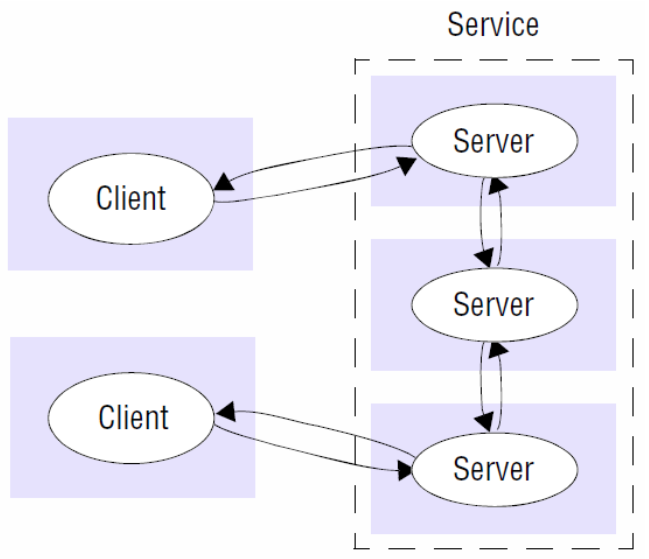
\includegraphics[width=\textwidth]{clientServer.png}
                \end{center}
            \end{column}
        \end{columns}
    \end{frame}

    \section{RPC, RMI}

    \begin{frame}
        \frametitle{RPC}
        \begin{center}
            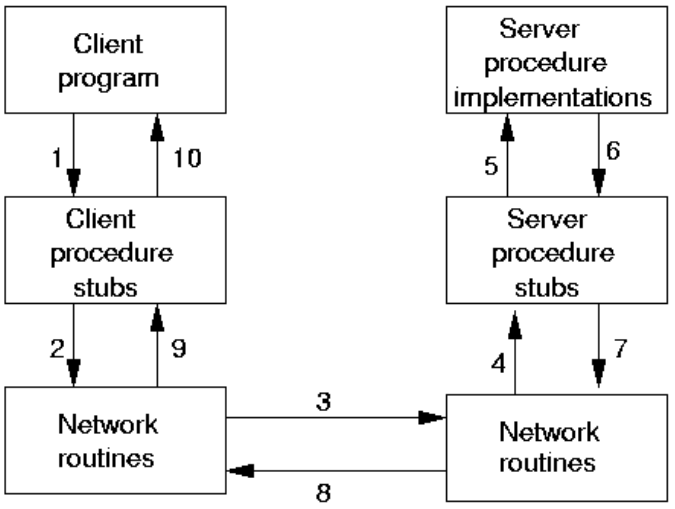
\includegraphics[width=0.6\textwidth]{rpc.png}
        \end{center}
    \end{frame}

    \begin{frame}
        \frametitle{Прозрачность RPC-вызовов}
        \begin{itemize}
            \item Изначальная цель --- максимальная похожесть на обычные вызовы
            \begin{itemize}
                \item Location and access transparency
            \end{itemize}
            \item Удалённые вызовы более уязвимы к отказам
            \begin{itemize}
                \item Нужно понимать разницу между отказом сети и отказом сервиса
                \begin{itemize}
                    \item Exponential backoff
                \end{itemize}
                \item Клиенты должны знать о задержках при передаче данных
                \begin{itemize}
                    \item Возможность прервать вызов
                \end{itemize}
            \end{itemize}
            \item Явная маркировка удалённых вызовов?
            \begin{itemize}
                \item Прозрачность синтаксиса
                \item Явное отличие в интерфейсах
                \begin{itemize}
                    \item Указание сематики вызова
                \end{itemize}
            \end{itemize}
        \end{itemize}
    \end{frame}

    \begin{frame}
        \frametitle{RMI}
        \begin{itemize}
            \item Локальные и удалённые объекты
            \item Интерфейсы удалённых объектов
            \item Ссылки на удалённые объекты
            \begin{itemize}
                \item Как параметры или результаты удалённых вызовов
            \end{itemize}
            \item Умеют исключения
        \end{itemize}
        \begin{center}
            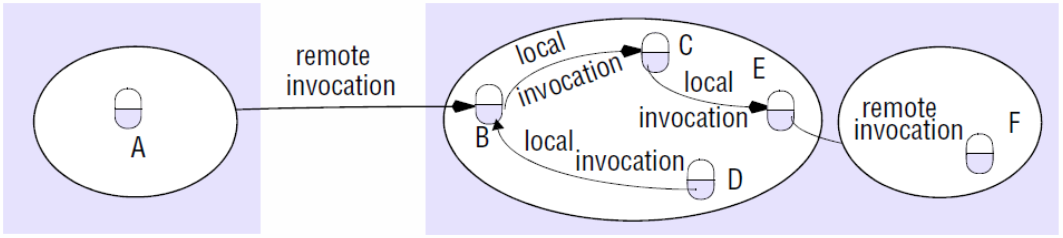
\includegraphics[width=0.8\textwidth]{remoteCalls.png}
        \end{center}
    \end{frame}

    \section{protobuf}

    \begin{frame}
        \frametitle{Protocol buffers}
        \framesubtitle{protobuf}
        \begin{itemize}
            \item Механизм сериализации-десериализации данных
            \item Компактное бинарное представление
            \item Декларативное описание формата данных, генерация кода для языка программирования
            \begin{itemize}
                \item Поддерживается Java, Python, Kotlin, Objective-C, C++, Go, Ruby, C\#, Dart
            \end{itemize}
            \item Бывает v2 и v3, с некоторыми синтаксическими отличиями
            \item Хитрый протокол передачи, \url{https://developers.google.com/protocol-buffers/docs/encoding}
            \begin{itemize}
                \item До 10 раз компактнее XML 
            \end{itemize}
        \end{itemize}
    \end{frame}

    \begin{frame}[fragile]
        \frametitle{Пример}
        Файл .proto:
        \begin{minted}{protobuf}
syntax = "proto3";

message Person {
    string name = 1;
    int32 id = 2;
    string email = 3;
}
        \end{minted}
        \vspace{2mm}
        Файл .java:
        \begin{minted}{java}
Person john = Person.newBuilder()
    .setId(1234)
    .setName("John Doe")
    .setEmail("jdoe@example.com")
    .build();
output = new FileOutputStream(args[0]);
john.writeTo(output);
        \end{minted}
    \end{frame}

    \section{gRPC}

    \begin{frame}
        \frametitle{gRPC}
        \begin{columns}
            \begin{column}{0.6\textwidth}
                \begin{itemize}
                    \item Средство для удалённого вызова (RPC)
                    \item Работает поверх protobuf
                    \item Тоже от Google, поддерживает те же языки, что и protobuf
                    \item Весьма популярен
                \end{itemize}
            \end{column}
            \begin{column}{0.4\textwidth}
                \begin{center}
                    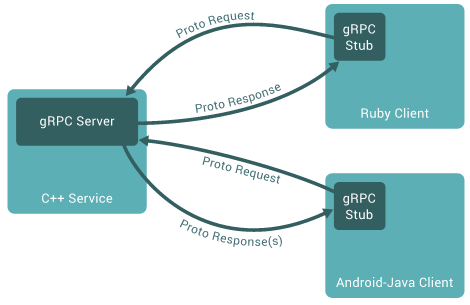
\includegraphics[width=\textwidth]{grpc.png}
                \end{center}
            \end{column}
        \end{columns}
    \end{frame}

    \begin{frame}[fragile]
        \frametitle{Технические подробности}
        \begin{itemize}
            \item Сервисы описываются в том же .proto-файле, что и протокол protobuf-а
            \item В качестве типов параметров и результатов --- message-и protobuf-а
        \end{itemize}
        \begin{minted}{protobuf}
service RouteGuide {
  rpc GetFeature(Point) returns (Feature) {}
  rpc ListFeatures(Rectangle) returns (stream Feature) {}
  rpc RecordRoute(stream Point) returns (RouteSummary) {}
  rpc RouteChat(stream RouteNote) returns (stream RouteNote) {}
}
        \end{minted}
        \attribution{\url{https://grpc.io/docs/languages/java/basics/}}
        \begin{itemize}
            \item Сборка --- плагином grpc к protoc
        \end{itemize}
\end{frame}

    \begin{frame}[fragile]
        \frametitle{Реализация сервиса на Java}
        \begin{scriptsize}
            \begin{minted}{java}
private static class RouteGuideService extends RouteGuideGrpc.RouteGuideImplBase {
    ...
    @Override
    public void getFeature(Point request, StreamObserver<Feature> responseObserver) {
      responseObserver.onNext(checkFeature(request));
      responseObserver.onCompleted();
    }

    @Override
    public void listFeatures(Rectangle request, StreamObserver<Feature> responseObserver) {
      for (Feature feature : features) {
        ...
        int lat = feature.getLocation().getLatitude();
        int lon = feature.getLocation().getLongitude();
        if (lon >= left && lon <= right && lat >= bottom && lat <= top) {
          responseObserver.onNext(feature);
        }
      }
      responseObserver.onCompleted();
    }
}
            \end{minted}
        \end{scriptsize}
    \end{frame}

    \begin{frame}[fragile]
        \frametitle{Реализация сервиса на Java (2)}
        \begin{scriptsize}
            \begin{minted}{java}
    @Override
    public StreamObserver<RouteNote> routeChat(
            final StreamObserver<RouteNote> responseObserver) {
      return new StreamObserver<RouteNote>() {
        @Override
        public void onNext(RouteNote note) {
          List<RouteNote> notes = getOrCreateNotes(note.getLocation());
          for (RouteNote prevNote : notes.toArray(new RouteNote[0])) {
            responseObserver.onNext(prevNote);
          }
          notes.add(note);
        }
        @Override
        public void onError(Throwable t) {
          logger.log(Level.WARNING, "routeChat cancelled");
        }
        @Override
        public void onCompleted() {
          responseObserver.onCompleted();
        }
      };
    }
            \end{minted}
        \end{scriptsize}
    \end{frame}

    \begin{frame}[fragile]
        \frametitle{Реализация клиента на Java (1)}
        \begin{scriptsize}
            \begin{minted}{java}
public RouteGuideClient(String host, int port) {
    this(ManagedChannelBuilder.forAddress(host, port).usePlaintext(true));
}

public RouteGuideClient(ManagedChannelBuilder<?> channelBuilder) {
    channel = channelBuilder.build();
    blockingStub = RouteGuideGrpc.newBlockingStub(channel);
    asyncStub = RouteGuideGrpc.newStub(channel);
}
            \end{minted}
        \end{scriptsize}
    \end{frame}

    \begin{frame}[fragile]
        \frametitle{Реализация клиента на Java (2)}
        \begin{scriptsize}
            \begin{minted}{java}
public void getFeature(int lat, int lon) {
    Point request = Point.newBuilder().setLatitude(lat).setLongitude(lon).build();
    Feature feature;
    try {
        feature = blockingStub.getFeature(request);
    } catch (StatusRuntimeException e) {
        warning("RPC failed: {0}", e.getStatus());
        return;
    }
    if (RouteGuideUtil.exists(feature)) {
        info("Found feature called \"{0}\" at {1}, {2}",
            feature.getName(),
            RouteGuideUtil.getLatitude(feature.getLocation()),
            RouteGuideUtil.getLongitude(feature.getLocation()));
    } else {
        info("Found no feature at {0}, {1}",
            RouteGuideUtil.getLatitude(feature.getLocation()),
            RouteGuideUtil.getLongitude(feature.getLocation()));
    }
}
            \end{minted}
        \end{scriptsize}
    \end{frame}

    \section{Веб-сервисы}

    \begin{frame}
        \frametitle{Веб-сервисы}
        \begin{itemize}
            \item Каждый веб-сервис --- отдельная система, представляющая что-то вроде RPC/RMI интерфейса
            \item Cложные приложения как интеграция веб-сервисов
            \item HTTP-запрос для выполнения команды
            \begin{itemize}
                \item Aсинхронное взаимодействие
                \item Ответ-запрос
                \item Событийные схемы
            \end{itemize}
            \item XML или JSON как основной формат сообщений
            \begin{itemize}
                \item SOAP/WSDL/UDDI
                \item XML-RPC
                \item REST
            \end{itemize}
        \end{itemize}
    \end{frame}

    \begin{frame}
        \frametitle{SOAP-ориентированные сервисы}
        \begin{columns}
            \begin{column}{0.6\textwidth}
                \begin{itemize}
                    \item Simple Object Access Protocol
                    \item Web Services Description Language
                    \item Universal Discovery, Description and Integration
                \end{itemize}
            \end{column}
            \begin{column}{0.4\textwidth}
                \begin{center}
                    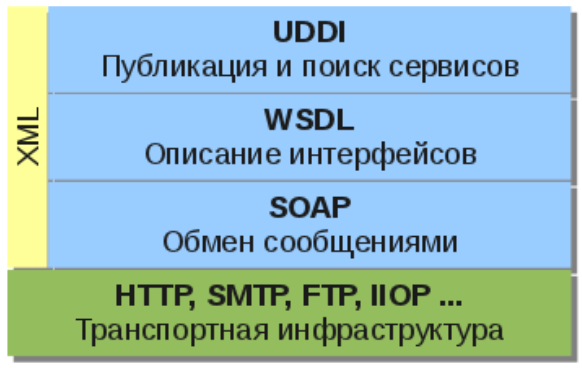
\includegraphics[width=\textwidth]{soap.png}
                \end{center}
            \end{column}
        \end{columns}
    \end{frame}

    \begin{frame}[fragile]
        \frametitle{SOAP-сообщение}
        \begin{small}
            \begin{minted}{xml}
<env:Envelope xmlns:env="http://www.w3.org/2003/05/soap-envelope">
    <env:Header>
        <n:alertcontrol xmlns:n="http://example.org/alertcontrol">
            <n:priority>1</n:priority>
            <n:expires>2001-06-22T14:00:00-05:00</n:expires>
        </n:alertcontrol>
    </env:Header>
    <env:Body>
        <m:alert xmlns:m="http://example.org/alert">
            <m:msg>Get up at 6:30 AM</m:msg>
        </m:alert>
    </env:Body>
</env:Envelope>
            \end{minted}
        \end{small}
    \end{frame}

    \begin{frame}[fragile]
        \frametitle{WSDL-описание}
        \begin{small}
            \begin{minted}{xml}
<message name="getTermRequest">
    <part name="term" type="xs:string"/>
</message>

<message name="getTermResponse">
    <part name="value" type="xs:string"/>
</message>

<portType name="glossaryTerms">
    <operation name="getTerm">
        <input message="getTermRequest"/>
        <output message="getTermResponse"/>
    </operation>
</portType>
            \end{minted}
        \end{small}
    \end{frame}

    \begin{frame}
        \frametitle{Достоинства SOAP-based сервисов}
        \begin{itemize}
            \item Автоматический режим описания сервисов
            \item Автоматическая поддержка описаний SOAP-клиентом
            \item Автоматическая валидация сообщений
            \begin{itemize}
                \item Валидность xml
                \item Проверка по схеме
                \item Проверка SOAP-сервером
            \end{itemize}
            \item Работа через HTTP
            \begin{itemize}
                \item Хоть через обычный GET
            \end{itemize}
        \end{itemize}
    \end{frame}

    \begin{frame}
        \frametitle{Недостатки SOAP-based сервисов}
        \begin{itemize}
            \item Огромный размер сообщений
            \item Сложность описаний на клиенте и сервере
            \item Один запрос --- один ответ
            \begin{itemize}
                \item Поддержка транзакций на уровне бизнес-логики
            \end{itemize}
            \item Сложности миграции при изменении описания
        \end{itemize}
    \end{frame}

    \section{WCF}

    \begin{frame}
        \frametitle{Пример: WCF}
        \frametitle{Windows Communication Foundation}
        \begin{itemize}
            \item Платформа для создания веб-сервисов
            \item Часть .NET Framework, начиная с 3.0
            \begin{itemize}
                \item Сейчас замещается ASP.NET Web APIs 
            \end{itemize}
            \item Умеет WSDL, SOAP и т.д., очень конфигурируема
            \item Автоматическая генерация заглушек на стороне клиента
            \item ABCs of WCF: Address, Binding, Contract
        \end{itemize}
        \begin{center}
            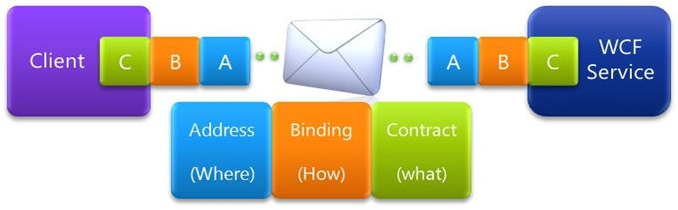
\includegraphics[width=0.6\textwidth]{wcf.png}
            \attribution{\url{http://www.c-sharpcorner.com}}
        \end{center}
    \end{frame}

    \begin{frame}[fragile]
        \frametitle{Пример, описание контракта}
        \begin{small}
            \begin{minted}{csharp}
[ServiceContract(Namespace = "http://Microsoft.ServiceModel.Samples")]  
public interface ICalculator  
{
    [OperationContract]
    double Add(double n1, double n2);

    [OperationContract]
    double Subtract(double n1, double n2);

    [OperationContract]
    double Multiply(double n1, double n2);

    [OperationContract]
    double Divide(double n1, double n2);
}
            \end{minted}
        \end{small}
    \end{frame}

    \begin{frame}[fragile]
        \frametitle{Пример, реализация контракта}
        \begin{small}
            \begin{minted}{csharp}
public class CalculatorService : ICalculator  
{
    public double Add(double n1, double n2)
        => n1 + n2;  

    public double Subtract(double n1, double n2)
        => n1 - n2

    public double Multiply(double n1, double n2)  
        => n1 * n2;

    public double Divide(double n1, double n2)  
        => n1 / n2;
}
            \end{minted}
        \end{small}
    \end{frame}

    \begin{frame}[fragile]
        \frametitle{Пример, self-hosted service}
        \begin{scriptsize}
            \begin{minted}{csharp}
Uri baseAddress = new Uri("http://localhost:8000/ServiceModelSamples/Service");
ServiceHost selfHost = new ServiceHost(typeof(CalculatorService), baseAddress);

try {
    selfHost.AddServiceEndpoint(typeof(ICalculator), new WSHttpBinding(), "CalculatorService");

    ServiceMetadataBehavior smb = new ServiceMetadataBehavior();
    smb.HttpGetEnabled = true;
    selfHost.Description.Behaviors.Add(smb);

    selfHost.Open();
    Console.WriteLine("The service is ready. Press <ENTER> to terminate service.");
    Console.ReadLine();

    selfHost.Close();  
} catch (CommunicationException ce) {
    Console.WriteLine($"An exception occurred: {ce.Message}");
    selfHost.Abort();
}
            \end{minted}
        \end{scriptsize}
    \end{frame}

    \begin{frame}[fragile]
        \frametitle{Пример, клиент}
        \begin{itemize}
            \item Генерация заглушки: 
                \begin{scriptsize}
                    \begin{minted}{text}
svcutil.exe /language:cs /out:generatedProxy.cs /config:app.config^
    http://localhost:8000/ServiceModelSamples/service
                    \end{minted}
                \end{scriptsize}
            \item Клиент:
                \begin{footnotesize}
                    \begin{minted}{csharp}

var client = new CalculatorClient();

double value1 = 100.00D;
double value2 = 15.99D;
double result = client.Add(value1, value2);
Console.WriteLine($"Add({value1},{value2}) = {result}");

client.Close();
                    \end{minted}
                \end{footnotesize}
        \end{itemize}
    \end{frame}

    \begin{frame}[fragile]
        \frametitle{Пример, конфигурация клиента}
        \begin{ssmall}
            \begin{minted}{xml}
<?xml version="1.0" encoding="utf-8" ?>  
<configuration>  
    <startup>   
      <!-- specifies the version of WCF to use-->  
        <supportedRuntime version="v4.0" sku=".NETFramework,Version=v4.5,Profile=Client" />  
    </startup>  
    <system.serviceModel>  
        <bindings>  
            <!-- Uses wsHttpBinding-->  
            <wsHttpBinding>  
                <binding name="WSHttpBinding_ICalculator" />  
            </wsHttpBinding>  
        </bindings>  
        <client>  
            <!-- specifies the endpoint to use when calling the service -->  
            <endpoint address="http://localhost:8000/ServiceModelSamples/Service/CalculatorService"  
                binding="wsHttpBinding" bindingConfiguration="WSHttpBinding_ICalculator"  
                contract="ServiceReference1.ICalculator" name="WSHttpBinding_ICalculator">  
                <identity>  
                    <userPrincipalName value="migree@redmond.corp.microsoft.com" />  
                </identity>  
            </endpoint>  
        </client>  
    </system.serviceModel>  
</configuration>
            \end{minted}
        \end{ssmall}
    \end{frame}

    \section{Очереди сообщений}

    \begin{frame}
        \frametitle{Очереди сообщений}
        \begin{itemize}
            \item Используются для гарантированной доставки сообщений
            \begin{itemize}
                \item Даже если отправитель и получатель доступны в разное время
                \item Локальное хранилище сообщений на каждом устройстве
            \end{itemize}
            \item Реализуют модель ``издатель-подписчик'', но могут работать и в режиме ``точка-точка''
            \item Как правило, имеют развитые возможности маршрутизации, фильтрации и преобразования сообщений
            \begin{itemize}
                \item Разветвители, агрегаторы, преобразователи порядка
            \end{itemize}
        \end{itemize}
    \end{frame}

    \section{RabbitMQ}

    \begin{frame}
        \frametitle{RabbitMQ}
        \begin{itemize}
            \item Сервер и клиенты системы надёжной передачи сообщений
            \begin{itemize}
                \item Сообщение посылается на сервер и хранится там, пока его не заберут
                \item Продвинутые возможности по маршрутизации сообщений
            \end{itemize}
            \item Реализует протокол AMQP (Advanced Message Queuing Protocol), но может использовать и другие протоколы
            \item Сервер написан на Erlang, клиентские библиотеки доступны для практически чего угодно
        \end{itemize}
        \begin{textblock}{3}(8,0)
            
\includegraphics[width=\textwidth]{rabbitmqLogo.png}
        \end{textblock}
    \end{frame}

    \begin{frame}[fragile]
        \frametitle{Пример, отправитель}
        \begin{ssmall}
            \begin{minted}{csharp}
using System;
using RabbitMQ.Client;
using System.Text;

var factory = new ConnectionFactory() { HostName = "localhost" };
using var connection = factory.CreateConnection();
using var channel = connection.CreateModel();
channel.QueueDeclare(queue: "hello", durable: false, exclusive: false,
        autoDelete: false, arguments: null);

string message = "Hello World!";
var body = Encoding.UTF8.GetBytes(message);

channel.BasicPublish(exchange: "", routingKey: "hello",
        basicProperties: null, body: body);
            \end{minted}
        \end{ssmall}
    \end{frame}

    \begin{frame}[fragile]
        \frametitle{Пример, получатель}
        \begin{ssmall}
            \begin{minted}{csharp}
using RabbitMQ.Client;
using RabbitMQ.Client.Events;
using System;
using System.Text;

var factory = new ConnectionFactory() { HostName = "localhost" };
using var connection = factory.CreateConnection();
using var channel = connection.CreateModel();
channel.QueueDeclare(queue: "hello", durable: false, exclusive: false, autoDelete: false, arguments: null);

var consumer = new EventingBasicConsumer(channel);
consumer.Received += (model, ea) =>
{
    var body = ea.Body;
    var message = Encoding.UTF8.GetString(body);
    Console.WriteLine(" [x] Received {0}", message);
};
channel.BasicConsume(queue: "hello", autoAck: true, consumer: consumer);
            \end{minted}
        \end{ssmall}
    \end{frame}

    \section{Apache Kafka}

    \begin{frame}
        \frametitle{Apache Kafka}
        \begin{itemize}
            \item Несколько другой подход к очередям: лог событий
            \begin{itemize}
                \item Сообщение посылается на сервер и хранится там вечно (ну, почти), получатель при обработке его не удаляет
                \item Индекс текущего сообщения хранит сам получатель, может отмотать назад
                \item Подход ``Event Sourcing'' --- не храним состояние, храним набор событий, позволяющих его получить
                \item Гораздо лучше с распределённостью
            \end{itemize}
            \item Быстрее RabbitMQ, лучше масштабируется
            \item Хуже с маршрутизацией (по идее), немного сложнее в настройке
        \end{itemize}
        \begin{textblock}{3}(8,0)
            
\includegraphics[width=\textwidth]{kafkaLogo.png}
        \end{textblock}
    \end{frame}

    \begin{frame}
        \frametitle{Apache Kafka, устройство}
        \begin{center}
            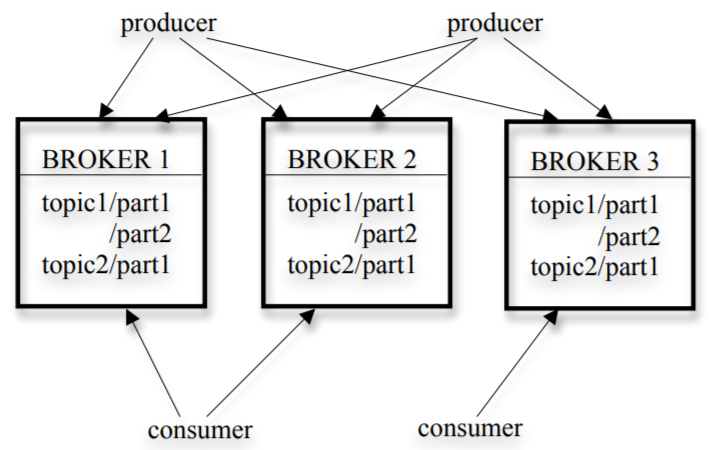
\includegraphics[width=0.6\textwidth]{kafkaArchitecture.png}
            \attribution{J. Kreps et al., Kafka: a Distributed Messaging System for Log Processing, 2011}
        \end{center}
        \begin{itemize}
            \item Топики --- каналы, куда можно писать
            \item Разделы --- логические куски топиков
            \item Брокеры --- отдельные сервера, балансируют нагрузку
            \item Сегменты --- файлы на диске, куски разделов, хранящиеся у брокеров
        \end{itemize}
    \end{frame}

    \begin{frame}[fragile]
        \frametitle{Пример, отправитель}
        \begin{small}
            \begin{minted}{csharp}
using Confluent.Kafka;

var config = new ProducerConfig { BootstrapServers = "localhost:9092" };

using var p = new ProducerBuilder<Null, string>(config).Build();
try
{
    var deliveryResult = await p.ProduceAsync(
        "test-topic", new Message<Null, string> { Value = "test" });
}
catch (ProduceException<Null, string> e)
{
    Console.WriteLine($"Delivery failed: {e.Error.Reason}");
}
            \end{minted}
        \end{small}
    \end{frame}

    \begin{frame}[fragile]
        \frametitle{Пример, получатель}
        \begin{ssmall}
            \begin{minted}{csharp}
using Confluent.Kafka;

var conf = new ConsumerConfig {
    GroupId = "test-consumer-group",
    BootstrapServers = "localhost:9092",
    AutoOffsetReset = AutoOffsetReset.Earliest
};

using var consumer = new ConsumerBuilder<Ignore, string>(conf).Build();
consumer.Subscribe("my-topic");

var cts = new CancellationTokenSource();
Console.CancelKeyPress += (_, e) => {
    e.Cancel = true;
    cts.Cancel();
};

try {
    while (true) {
        var consumeResult = consumer.Consume(cts.Token);
        Console.WriteLine($"Consumed message '{consumeResult.Message.Value}'.");
    }
}
catch (OperationCanceledException) {
    consumer.Close();
}
            \end{minted}
        \end{ssmall}
    \end{frame}

\end{document}
